\makeatletter\let\ifGm@compatii\relax\makeatother 
\documentclass{beamer}

%-----------------------------------------------------------------------------------------

\usepackage{pgfarrows,pgfnodes,pgfautomata,pgfheaps,tikz}
\usepackage{amsmath,amssymb}
\usepackage{color}
\usepackage[utf8]{inputenc}
\usepackage{ae}
\usepackage{xspace}
\usepackage{courier}

\usepackage{listings}
\usepackage{color}

%-----------------------------------------------------------------------------------------


\setbeamertemplate{background canvas}[vertical shading][bottom=red!10,top=blue!10]
% \usetheme{Warsaw}
\usetheme{default}
\usefonttheme[onlysmall]{structurebold}
\setbeamercovered{dynamic}

%-----------------------------------------------------------------------------------------

\title[Ciencia de Datos]{\\\large{Introducci\'on a Ciencia de Datos}}
%\date[DLT 2003]{17/03/2016}
\date[DLT 2003]{}

%-----------------------------------------------------------------------------------------

\begin{document}

%-----------------------------------------------------------------------------------------

\frame{\titlepage}

% Especificar el origen del curso original
\begin {frame}
\frametitle{Organizaci\'on del curso}
	\begin{itemize}
	\item Introducci\'on a Ciencia de Datos y Big Data
	\item Manejo de archivos/Expresiones regulares
	\item Scraping de la Web/Manipulación de datos
	\item Modelo Relacional: Modelización/Normalización
	\item Técnica Map-Reduce
	\item Bases de Datos NoSQL
	\item Estadística y probabilidad
	\item Técnicas de Aprendizaje Automático (Machine Learning)
	\item Visualización
	\end{itemize}

\end{frame}

\begin {frame}

\frametitle{Agradecimientos}
\begin{itemize}
	\item Este curso es una versi\'on libre del curso on-line \\
			Introducci\'on a la Ciencia de Datos (Bill Howe, Univ. de \\
			Wasshington) \href{url}{https://www.coursera.org/course/datasci}
	\item CS109 Data Science (Harvard Univ.)
	\item El Dr. Esteban Feuerstein nos facilit\'o parte del material \\
			introductorio
			
\end{itemize}
\end{frame}

\begin {frame}
\frametitle{Definici\'on informal}

``La Ciencia de Datos es un \'area de trabajo nueva vinculada a la 
recolecci\'on, adaptaci\'on, an\'alisis, visualizaci\'on y 
preservaci\'on de grandes vol\'umenes de datos" (An Introduction to 
Data Science, Jeffrey Stanton)

\end{frame}

\begin {frame}

La Ciencia de Datos aparece en el cruce de 3 \'areas:
	\begin{itemize}
	\item Procesamiento de datos (depuraci\'on y formateo de datos)
	\item T\'ecnicas de aprendizaje autom\'atico y estadística
	\item Visualizaci\'on (comunicar los resultados)
	\end{itemize}

\end{frame}

\begin {frame}

\frametitle{La Ciencia de Datos y los \emph{Productos de Datos}}

La Ciencia de Datos no s\'olo se ocupa de responder preguntas
tambi\'en se ocupa de hacer aplicaciones (\emph{Productos de Datos})

\bigskip

Algunos ejemplos:
	\begin{itemize}
	\item Aplicaciones de Datos (correctores ortogr\'aficos,
	traductores)
	\item Visualizaciones interactivas (Google Maps, Mapa de la Gripe)
	\item Bases de Datos on-line (Sloan Digital Sky Survey)
	\end{itemize}

\end{frame}


\begin{frame}

\frametitle{Campa\~nas electorales}
	En la actualidad se emplean metodolog\'ias de an\'alisis
	de datos para definir los distintos grupos socioculturales a los
	cuales se trata de influir durante las campa\~nas electorales

\end{frame}

\begin{frame}

\frametitle{Resignificar la informaci\'on}

	Emplear la informaci\'on disponible en internet de formas novedosas
	
\begin{itemize}
	\item Ejemplo: Hurac\'an Sandy tomar informaci\'on de estaciones
	meteorol\'ogicas y producir una visualizaci\'on en tiempo real del
	paso del hurac\'an
\end{itemize}

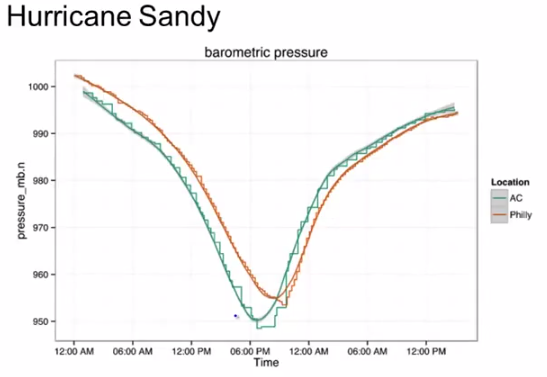
\includegraphics[scale=.4]{img/huracan.png}

\end{frame}

\begin{frame}

\frametitle{An\'alisis de emociones en textos}
%(8:04)
\begin{enumerate}%[<+->]
	\item Convertir todos los libros digitalizados a n-gramas (Google \\
	\href{url}{https://books.google.com/ngrams})
	\begin{itemize}
		\item 1-grama: "Inflaci\'on"
		\item 6-grama: "El costo de vida aumenta diariamente"
	\end{itemize}
	\item Asignarle a cada 1-grama un puntaje ``emocional" (WordNet \\
	\href{url}{https://wordnet.princeton.edu/})
	\item Contar y normalizar las ocurrencias de cada palabra
\end{enumerate}

\end{frame}


\begin{frame}
\frametitle{An\'alisis de emociones en textos}
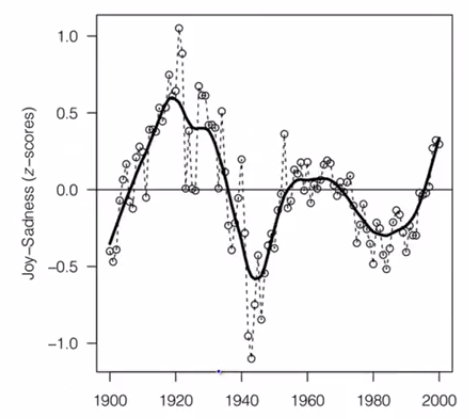
\includegraphics[scale=.5]{img/afect1.png}
\end{frame}

\begin{frame}
\frametitle{An\'alisis de emociones en textos}
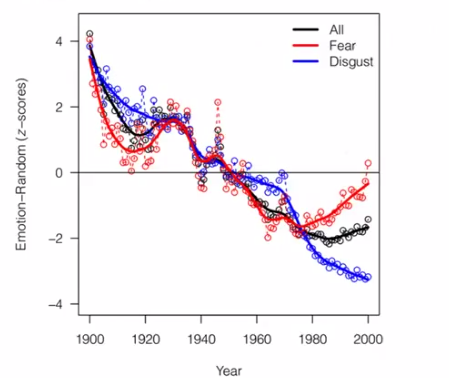
\includegraphics[scale=.5]{img/afect2.png}
\end{frame}


\begin {frame}

La Ciencia de Datos est\'a revolucionando otras \'areas
	\begin{itemize}
	\item M\'etodos novedosos de an\'alisis de datos se emplean en 
	ciencias sociales: historia, antropolog\'ia, lingü\'istica
	\item El periodismo de investigaci\'on (Wikileaks)
	\end{itemize}

\end{frame}

%1-2
\begin{frame}

\frametitle{Casos de error}
	Se produjo un error en la estimaci\'on del pico de gripe a partir 
	de las consultas en Google porque la prensa le dio difusi\'on y se 
	magnific\'o la intensidad
\end{frame}

%1-3

%1-4
%1-5
%1-6

\begin {frame}

``El mayor obst\'aculo en el procesamiento de datos proviene de la gran 
variedad de formatos existentes, de la informaci\'on no estructurada y 
de las fuentes contradictorias." (Doug Laney)

\end{frame}

%1-7

\begin {frame}
\frametitle{eScience}

\emph{eScience} es una nueva perspectiva en las ciencias emp\'iricas 
seg\'un la cual se capturan datos masivamente para emplearlos en la 
verificaci\'on de las hip\'otesis cient\'ificas.

\bigskip

Gracias a los avances tecnol\'ogicos recientes se abarat\'o mucho el 
costo de la obtenci\'on de datos.

\bigskip

El ritmo al que se producen los datos supera ampliamente nuestra 
capacidad actual para analizarlos.

\end{frame}

\begin{frame}
\frametitle{eScience: Astronom\'ia}
Es posible hacer mapeos peri\'odicos de la galaxia en alta resoluci\'on
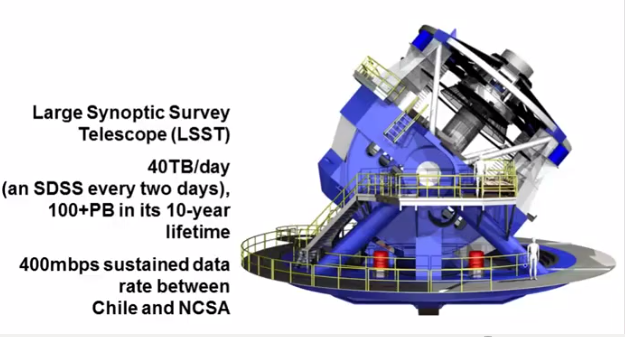
\includegraphics[scale=.5]{img/astronomia.png}
\end{frame}

\begin{frame}
\frametitle{eScience: Oceanograf\'ia}
Modelos de alta resoluci\'on, sensores baratos, sat\'elites
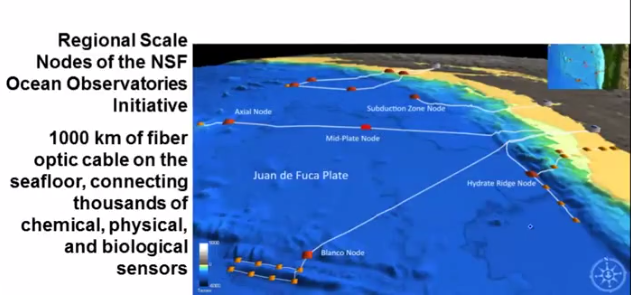
\includegraphics[scale=.5]{img/oceanografia.png}
\end{frame}

\begin{frame}

\frametitle{Internet}
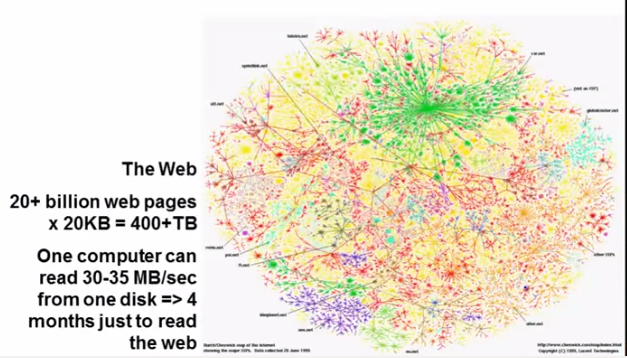
\includegraphics[scale=.5]{img/web.png}

\end{frame}

\begin{frame}

\frametitle{Big Data: una definici\'on informal}
``\emph{Big Data} es cualquier conjunto de datos costoso de mantener y 
dif\'icil de procesar." (Michael Franklin, Univ. Berkeley)

\end{frame}

\begin{frame}
\frametitle{Big Data: las 3 V's}
	\begin{itemize}
	\item Volumen: el tama\~no de los datos
	\item Velocidad: la relaci\'on entre el procesamiento de datos y la 
	creciente necesidad de interactividad (tiempo real)
	\item Variedad: la diversidad de fuentes de datos, formatos, 
	estructuras, etc.
	\end{itemize}
\end{frame}


\end{document}

	

	


